\chapter{Method for Experimental Work}
\label{chap:method}
%In this chapter the methodology for the creation of the two models will be described.
This chapter defines the methodology and approach of the experimental work conducted at Trondheim Biological Station. Aksel Alstad Mogstad, one of the experts, supervised the entire experiment with steady guidance. The approach describing the processing and analyses of the data, done at a later stage, is presented towards the end of the chapter.

\section{Laboratory Testing}

\subsection{The Set-Up}
Figure \ref{fig:lab-set-up} contain images of the components used in the laboratory experiment. The spectrometer (a) was turned on and connected to the software OceanView 1.6.7 via a standard external computer. In OceanView, the spectrometer was sat to a constant temperature of 15 degrees (Celsius). The QR400-7-VIS-BX reflection probe (b) was connected to the spectrometer through one cable, and a light source through another. The cables are fiber optic, and are assumed to not have a noteworthy effect the results. The light source used was Schott KL1500 electronic light source (c), a 150 W halogen light delivering a constant spectral signature - after given some time to heat up. In addition, the reflection probe was placed in a reflective probe holder (d), angling the light output (and the sensor inlet) in order to avoid specular reflection. This angle was sat to 45 degrees and the distance to 1 centimeter.
\\\\
Furthermore, the reflective probe was placed over the object to be measured (d). Initially, this was the WS-1 Reflectance Standards (e) with 100 percent reflectance within the range of 250-1500 nanometers. This was measured in OceanView and sat the standard for white. The reflectance was assumed to be 100\% for the reflectance standard. Note that this is the Lambertian surface mentioned in Section \ref{sec:specref}. The reflectance standard calibrate the software such that all further measurement will be a relative size compared to the original standard white. An effect of measurements being relative to the original white is the accounting of, and subsequent omittance of the noise due to the light source. 



\begin{figure}[H]
  \newcommand*\FigVSkip{0.5em}
  \newcommand*\FigHSkip{0.1em}
  \newsavebox\FigBox
  \centering
  % Top image is centered, so no need to get width
 \sbox{\FigBox}{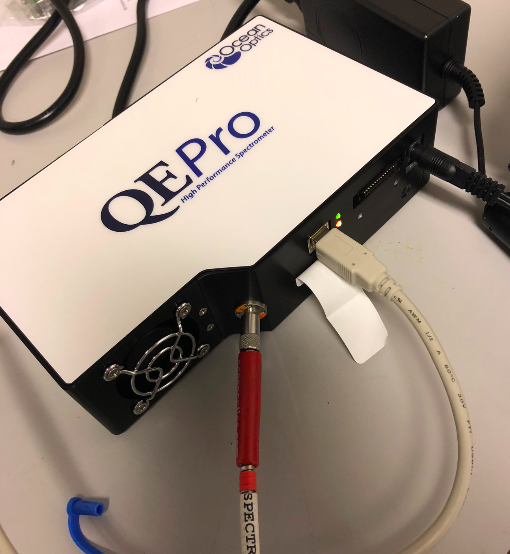
\includegraphics[height=5cm]{Images/method/qe-pro.png}}
  \begin{minipage}{\wd\FigBox}
    \centering\usebox{\FigBox}
    \subcaption{a) QE Pro}
  \end{minipage}
    % Top image is centered, so no need to get width
 \sbox{\FigBox}{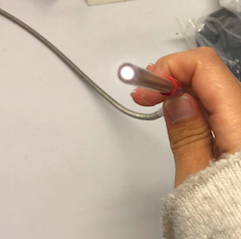
\includegraphics[height=5cm]{Images/method/light.png}}
  \begin{minipage}{\wd\FigBox}
    \centering\usebox{\FigBox}
    \subcaption{b) Reflection probe}
  \end{minipage}
  % Save first image in a box to get the width
  \sbox{\FigBox}{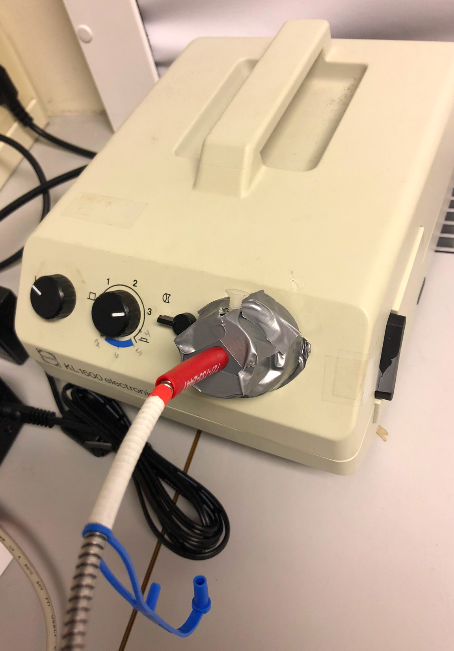
\includegraphics[height=5cm]{Images/method/lightsource.png}}
  \begin{minipage}{\wd\FigBox}
    \centering\usebox{\FigBox}
    \subcaption{c) Light source, Schott KL1500, 150 W halogen}
  \end{minipage}\hspace*{\FigHSkip}
  % Save second image 
\end{figure}

\begin{figure}[H]
  \newcommand*\FigVSkip{0.5em}
  \newcommand*\FigHSkip{0.1em}
  \newsavebox\FigBox
  \centering
  % Top image is centered, so no need to get width
 \sbox{\FigBox}{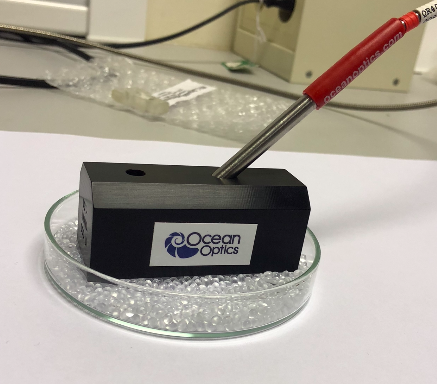
\includegraphics[height=4cm]{Images/method/setup.png}}
  \begin{minipage}{\wd\FigBox}
    \centering\usebox{\FigBox}
    \subcaption{d) Reflection probe holder from Ocean Optics}
  \end{minipage}
    % Top image is centered, so no need to get width
 \sbox{\FigBox}{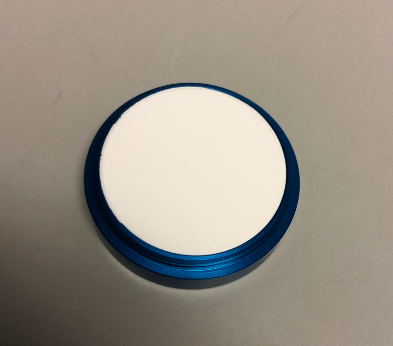
\includegraphics[height=4cm]{Images/method/lamber.png}}
  \begin{minipage}{\wd\FigBox}
    \centering\usebox{\FigBox}
    \subcaption{e) WS-1 Reflectance standard, lambertian surface from Ocean Optics}
  \end{minipage}
  % Save first image in a box to get the width
  \sbox{\FigBox}{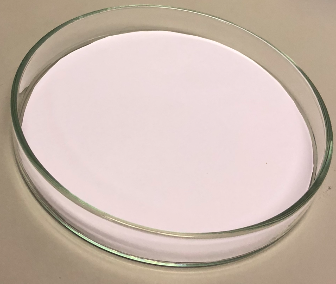
\includegraphics[height=4cm]{Images/appendix/papir.png}}
  \begin{minipage}{\wd\FigBox}
    \centering\usebox{\FigBox}
    \subcaption{f) Paper background}
  \end{minipage}\hspace*{\FigHSkip}
  % Save second image 
  \caption[The Laboratory Set-up]{The laboratory set-up}
  \label{fig:lab-set-up}
\end{figure}


\\\\
\noindent
In order to avoid further noise, the lab was kept as dark as possible to avoid ambient light. Light blocking blinds were used and to avoid the glare from the computer screen to affect the signature, the computer was covered behind a screen made of cardboard. Once the room was sufficiently dark, the spectrometer was turned on separately from the light source. This was done to measure the signal delivered from the sensor in completely dark environments. This dark noise could then be compensated for by the software. Throughout the experiment, the dark noise was only measured once - at the beginning of the experiment.
\\\\
Even though the reflectance standard is supposed to be 100\% reflective, there is still a possibility of achieving higher than 100\% which occurs in mirrors. The results would be saturation, which causes the measurement to flatten. As a consequence, one would lose information. As the plastic could contain mirror like properties, a margin was set in order to avoid saturation.
\\\\
Oceanview continuously sampled from the camera at a rate equivalent to the shutter speed - every 800 milliseconds. However, in order to obtain minimum amount of noise, the signature was more rarely updated. The software averaged the values obtained between each update. As a result, the obtained signature was an average of 5 scans. Therefore, the signature was updated every 4 seconds. As there should be no variation in the signature when measuring the same sample, the variation may be regarded as noise. 
\\\\
In addition, the delay in the system is irrelevant at this stage. This is due to the absence of a control system or other systems relying on delivering a real-time response to the signature.
\\\\
Going further, a layer of plastic was placed in a glass petridish with a double layer of white paper in the bottom. The layer of plastic was intended to be a single layer in order to see the effect of thickness on the see-through plastic. The petridish was used to contain the plastic, while the white paper was used to avoid the results of the see-through plastic to be affected by the background. The reflective probe holder was then placed over the specific plastic type to be measured. Each type of plastic was measured 10 times - each time a different place. The plastic types with variation in color was measured 10 times per color. This way, the different colored samples were possible to separate. The reflectance from the plastic pieces was then visualized in OceanView and ready for comparison. This process was iterated with different types of plastic. 
\\\\
The movement of the reflective probe holder can affect the scanner and thereby change the angle affecting the reflectance. In between samples and after conducting five samples of the same material, the the software was therefore calibrated with the standard white. Given the software’s relative measuring, this hopefully ensured the maintenance of correct reflectance for all signatures.

\subsection{Choice of Spectrum}
As discussed in Section \ref{lightinwater}, infrared and near-infrared light has a poor "performance" in water. Due to infrared and near-infrared light being low-energy it quickly disappears over a short distance in water. This will make it difficult to measure and could possibly result in large variations in the signature, which would be difficult to account for. This, in addition to information extracted from the water absorption figure, Figure \ref{fig:absspec} displayed in Section \ref{lightinwater}, point towards the visible light spectrum as the better alternative, underwater.
\\\\
Furthermore, higher wave lengths depicted high levels of noise and inconsistencies in the measured values. This was most likely due to the relative measurements of the software. The measured values are relative in the sense that the \textit{actual} measured value is divided by the reflective standard. The reflective standard yielded low values in the IR and NIR spectra. Since small values in the divisor cause large variations as it will be greatly multiplied, the variations were large. Also, UV-lighting and other light with wavelengths outside the visible spectrum were neglected.
\\\\
Because of all of the above, the visible spectrum was measured in the interval 400nm - 700nm. The resulting intensity was measured approximately every 0,758 nanometers. 

\section{Materials} \label{sec:material}
In order to cover a wide range of plastic, eventually turning into microplastic, the material tested were the most common types of plastic. Table \ref{tab:tested:plastic} shows the types of plastic tested, their state and additives:

\begin{center}
\begin{table}[H]
\begin{tabular}{ |l|l|l|l|l| }
 \hline
 \textbf{State} & \textbf{Class} & \textbf{Additives}\\ 
Post-Industrial Recyclate Pellets & PE: LDPE/LLDPE & Colorants \& printing inks\\
Post-Consumer Recyclate Regrind & PE-HD & Colorants\\
Environmental Pellets & PE: LDPE/HDPE & Yes, unspecified\\
Environmental Fragments (Regrind) & PE-HD & Yes, unspecified\\
Pristine Pellets & PP-Homopolymer & Stabilizers\\
Post Consumer Recyclate: Pellets & PP Mixture & Yes, unspecified\\
Pristine Pellets & PS General purpose & Unknown\\
Post Consumer Recyclate Regrind & PS Mixture & Yes, unspecified\\ 
Pristine Pellets & PET Amorphous & No intentional additives\\
Post Consumer Recyclate Regrind & PET Amorphous & No intentional additives\\
Pellets & PVC Soft & Yes, softener\\
Pellets & PVC Hard & Yes, softener \& mineral filler\\
 \hline
\end{tabular}
\caption{Table of tested plastic types}
\label{tab:tested:plastic}
\end{table}
\end{center}
\noindent
The plastic was ordered from at German supplier, CARAT GmbH, by recommendation from Andy Booth at the Environment and New Resources department at Sintef Ocean. This supplier was chosen as their material achieve high purity. In order to visualize differences in material due to additives and other alternations made by the manufacturers, the used samples are a mix of pure and recycled material. In addition to the ordered plastic, some household objects were measured. These include:
\\\\
\noindent
$\cdot$ Multicolored plastic bag - Red, Blue and White\\
$\cdot$ Black plastic bag\\
$\cdot$ Plastic bottle A - Transparent\\
$\cdot$ Plastic bottle B - Transparent\\
$\cdot$ Plastic bottle C - See-Through with Blue tint.
\\\\
Note: A more extensive list of the plastic samples can be found in Appendix \autoref{app:list_plast} while image of the samples may be found in Appendix \autoref{app:image_plast}.


\section{Data Processing and Analysis}
The data obtained from the laboratory testing were interpreted using PCA and the software Unscrambler X. The acquired data was exported to Microsoft Excel from Oceanview, where each cell represented the measured value at a given wavelength. The spreadsheet was subsequently made to fit the required structure of The Unscrambler X. The PCA was run using The Unscrambler X, while the results were visualized using a R-script. To assess the spectral relationship between different objects and materials, principal component analyses were performed on the laboratory-acquired reflectance data. 

%Underwater hyperspectral imaging: a new tool for marine archaeology 2018, ØYVIND ØDEGÅRD,1,2,* AKSEL ALSTAD MOGSTAD,3 GEIR JOHNSEN,3 ASGEIR J. SØRENSEN, AND MARTIN LUDVIGSEN1

\\\\
\noindent
Extracting information from the data acquired was done using the software \textit{The Unscrambler X 10.1}. The software is originally developed by Harald Martens, an adjunct professor at NTNU, and is a commercial software product for multivariate data analysis. The possible variables for the analysis were the wavelengths from the spectrometer and the size of the pellets. The software processes the data according to the principal described in Section \ref{sec:pca} in Chapter \ref{cap:theory3}. The analysis takes the data set as an input including the variables based on the formatting of the spreadsheet. 
\\\\
Subsequently, a standard Principal Component Analysis was ran using seven principal components and 100 iterations. With the use of two components, 97,8 \% were explained. Therefore, a third component, only complicating the visualization of the results, was not needed.
\\\\
Furthermore, an uncertainty test on the data, as well as a sampling test, was ran. The latter ran several analyses excluding different samples each time in order to see whether the data was consistent or not. The uncertainty test checked whether the data was within certain limits. These tests were based on the confidence interval from the Hotelling's $T^2$ plot described in Section \ref{sec:hotellings} from Chapter \ref{cap:theory3}. 
\\\\
Lastly, the results were visualized in a large number of plots generated by the software, letting the user assess the results more intuitively. 
\\\\
Due to the unproportional effect on the principal components of some samples, these were excluded from the analysis. As previously explained in the theory section of PCA, the principal components are measure based on the largest variance in the samples. Therefore, certain samples with unlikely values due to other effects will skew the result. This can result in the variance being almost fully explained by the change in one variable. This way, the results having an unproportionally high effect on the results, were excluded.
\\\\%Dette burde begrunnes i en hotelling's, da kan man vise residual og leverage
The previously mentioned samples which skewed the results, were identified using the Hotelling's $T^2$ VS Residual plot described in Section \ref{sec:vs} from Chapter \ref{cap:theory3}. This plot shows the samples having large deviation from the norm and a large deviation. The combination of the two shows the impact each samples have on the final result. Whenever a sample is abnormally far to the right, that sample influence the result much more than the rest of the dataset. As there was no explainable reason to why these samples had such an impact, the samples were removed from the dataset. After excluding these samples, the resulting explained percentage was 94,5 \%, with PC1 explaining 80,1 \% and PC2 13,4 \%. PC1 is still considerable, but less than before.
\\\\
The results from the PCA were visualized using R programming through a script. The script assigns each sample a color in the scatter and encloses the measurements in a 95 \% confidence interval. It also centers a circle in the origin which have vectors depicting the direction having a certain increasing color, i.e., a red arrow vector would represent the direction with an increasing red color component. Furthermore, the script visualize the contribution of the different wavelengths. The continuous graph changes color according to the corresponding wavelength. The line representing the average contribution is also represented. Given a sample every 0.758 nanometers and 300 possible wavelengths results in the line representing $100\% \cdot 0.758/300 \approx 0.253 \% $
\\\\
Using already existing dataset from crustaceans and algae, provided by one of the experts, Aksel Alstad Mogstad, it was possible to compare the dataset regarding plastic with similar measurements from microorganisms containing natural pigments. These are microorganisms that co-exist with plastic in a marine environment. The algae used were; brown algae, green algae and red coralline algae.
\\\\
When plotting the signatures of the associated type of plastic, the average of all ten samples were used. This was done in MATLAB. All signatures can be found in Appendix \ref{app:signatures}.
















\begin{comment}

\section{Hyperspectral Imaging} 
%evt bare spektrometeret - teste alle de ulike typene plast som vi har kjøpt fra tyskland 


\subsection{Purpose}
The purpose of the experiment is to get a better understanding of the properties of specific plastic types. By looking at how light is reflected from different types of plastic, it will be possible to compare the plastic types and hopefully detect some kind of pattern. Initially, the plastic pellets will be examined in a dry environment, before being placed in water later on. These results will be compared in order to see if experiments carried out in dry environment can be representative for plastic pellets in wet environment. 

\subsection{Hypotheses}
$\bullet$ Different types of plastic provide different signatures in the visible light spectrum\\ 
$\bullet$ Various types of plastic provide different signatures in infrared light spectrum\\
$\bullet$ Different types of plastic have different intensities of reflecting light\\
$\bullet$ Varying thickness in a specific type of plastic, will give different results\\
$\bullet$ Post consumer recycled pellets and clean pellets have different signatures\\
%Hvis dette stemmer, må vi finne ut om plasten noen gang kan anses som ”clean” i livsløpet (for eksempel på starten/etter hvert som farge osv er vasket av)
$\bullet$ The same type of plastic gives a similar signature in water as well as in a dry environment

\subsection{Material}
\begin{center}
\Rotatebox{0}{
\begin{tabular}{ |c|c|c|c|c| }
 \hline
 \textbf{Ref Number} & \textbf{State} & \textbf{Class} & \textbf{Additives} \\ 
 
 CRT131.00 & Post-Industrial Recyclate Pellets & PE: LDPE/LLDPE & Yes, colorants\\
 CRT150.00 & Post-Consumer Recyclate Regrind & PE-HD & Colorants \\
CRT170.00 & Environmental Pellets & PE: LDPE/HDPE & Yes \\
CRT171.00 & Environmental Fragments (Regrind) & PE-HD & Yes \\
CRT200.00 & Pristine Pellets & PP-Homopolymer & Yes, stabilizers \\
CRT250.00 & Post Consumer Recyclate: Pellets & PP Mixture & Yes \\
CRT300.00 & Pristine Pellets & PS General purpose & Unknown \\
CRT331.00 & Post Consumer Recyclate Regrind & PS Mixture & Yes \\
CRT400.00 & Pristine Pellets & PET Amorphous & No, not intentionally \\
CRT451.00 & Post Consumer Recyclate Regrind & PET Amorphous & No, not intentionally \\
CRT500.00 & Pellets & PVC Soft & Yes, softener \\
CRT530.00 & Pellets & PVC Hard & Yes, softener \\
 \hline
\end{tabular}
}
\end{center}
%$\bullet$ plastpose\\\\
%$\bullet$ plastflaske\\\\
%$\bullet$ …?

\subsection{Equipment} 
(from ocean optics web page)\\
$\bullet$ QE Pro spectrometer - measures optical signatures on the specific object. In this experiment, reflectance is used to illustrate the color properties\\
$\bullet$ WS-1 Reflectance Standards - 100 percent reflectance within 250-1500 nanometers\\
$\bullet$ QR400-7-VIS-BX reflection probe, light out and reflectance in\\
$\bullet$ RPH reflective probe holder, holding the reflection probe in a 45 degree angle and keeping the source 1 cm away from the measured object\\
$\bullet$ OceanView 1.6.7 - The program used to visualize the object reflectance \\
$\bullet$ Light source

\subsection{Procedure} 
The spectrometer is turned on and connected to OceanView 1.6.7 via an external computer. In OceanView, the spectrometer is set to a constant temperature of -10 degrees (Celsius). The QR400-7-VIS-BX reflection probe is connected to the spectrometer through one cable, and a light source through another. In addition, the reflection probe is placed in a reflective probe holder, angling the light output (and the sensor inlet) in order to avoid specular reflection. This angle is set to 45 degrees.
\\\\
Furthermore, the reflective probe is placed over the object to be measured. To begin with, this is the WS-1 Reflectance Standards with 100 percent reflectance within the range of 250-1500 nanometers. This is measured in OceanView and sets the standard for white. Furthermore, the reflective probe holder is placed over the specific plastic type to be measured. The reflectance from the plastic pieces is then visualized in OceanView and is ready for comparison. This process will be repeated with different types of plastic.
\\\\
%Underwater hyperspectral imaging: a new tool for marine archaeology 2018, ØYVIND ØDEGÅRD,1,2,* AKSEL ALSTAD MOGSTAD,3 GEIR JOHNSEN,3 ASGEIR J. SØRENSEN, AND MARTIN LUDVIGSEN1
We assume ideal lighting such that the measured radiance of an object is independent of its position on the scan line. Additionally, the reference plate is assumed to reflect the downwelling radiance equally at all wave- lengths. 

%Samme gjennomføres i vann?
%Samme gjennomføres med store plastbiter?

%Ønsket resultat?

\section{Underwater Hyperspectral Imaging} 

\section{Introducing a SilCam Lens} Implementere linsen i tidligere oppsett. 

\section{PCA} Denne baseres på dataen funnet fra metodene over: finner ut hvor sensitiv plasttypen er for forskjellige bølgelengder - er dette en plasttype som gir samme signatur over alle bølgelengder og er uniform feks?

\subsection{Classification} Herunder klassifisering og kategorisering - feks basert på signatur. (Leter etter en trender i datasettet.)

\section{Measurement of Success}
Målestokk for suksess

\end{comment}